% SECTION ====================================================================================
\section{Algorithmen und Datenstukturen}
% ============================================================================================

\begin{sectionbox}
\subsection{Terminologie}\par\smallskip
\textbf{Algorithmus}: Wohldefinierte Berechnungsvorschrift, welche aus Eingabedaten (input/Probleminstanz) Ausgabedaten (output) berechnet.\par\smallskip
\textbf{Datenstrukturen}: Eine Datenstruktur organisiert Daten so in einem Computer, dass man sie (in den
darauf operierenden Algorithmen) effizient nutzen kann.\par\smallskip
\textbf{Effizienz}: Die Effizienz eines Algorithmus ist seine Sparsamkeit bezüglich der Ressourcen, Zeit und Speicherplatz, die er zur Lösung eines festgelegten Problems beansprucht.
\end{sectionbox}

\begin{sectionbox}
\subsection{Effizienz von Algorithmen}\smallskip
%\begin{center}
%    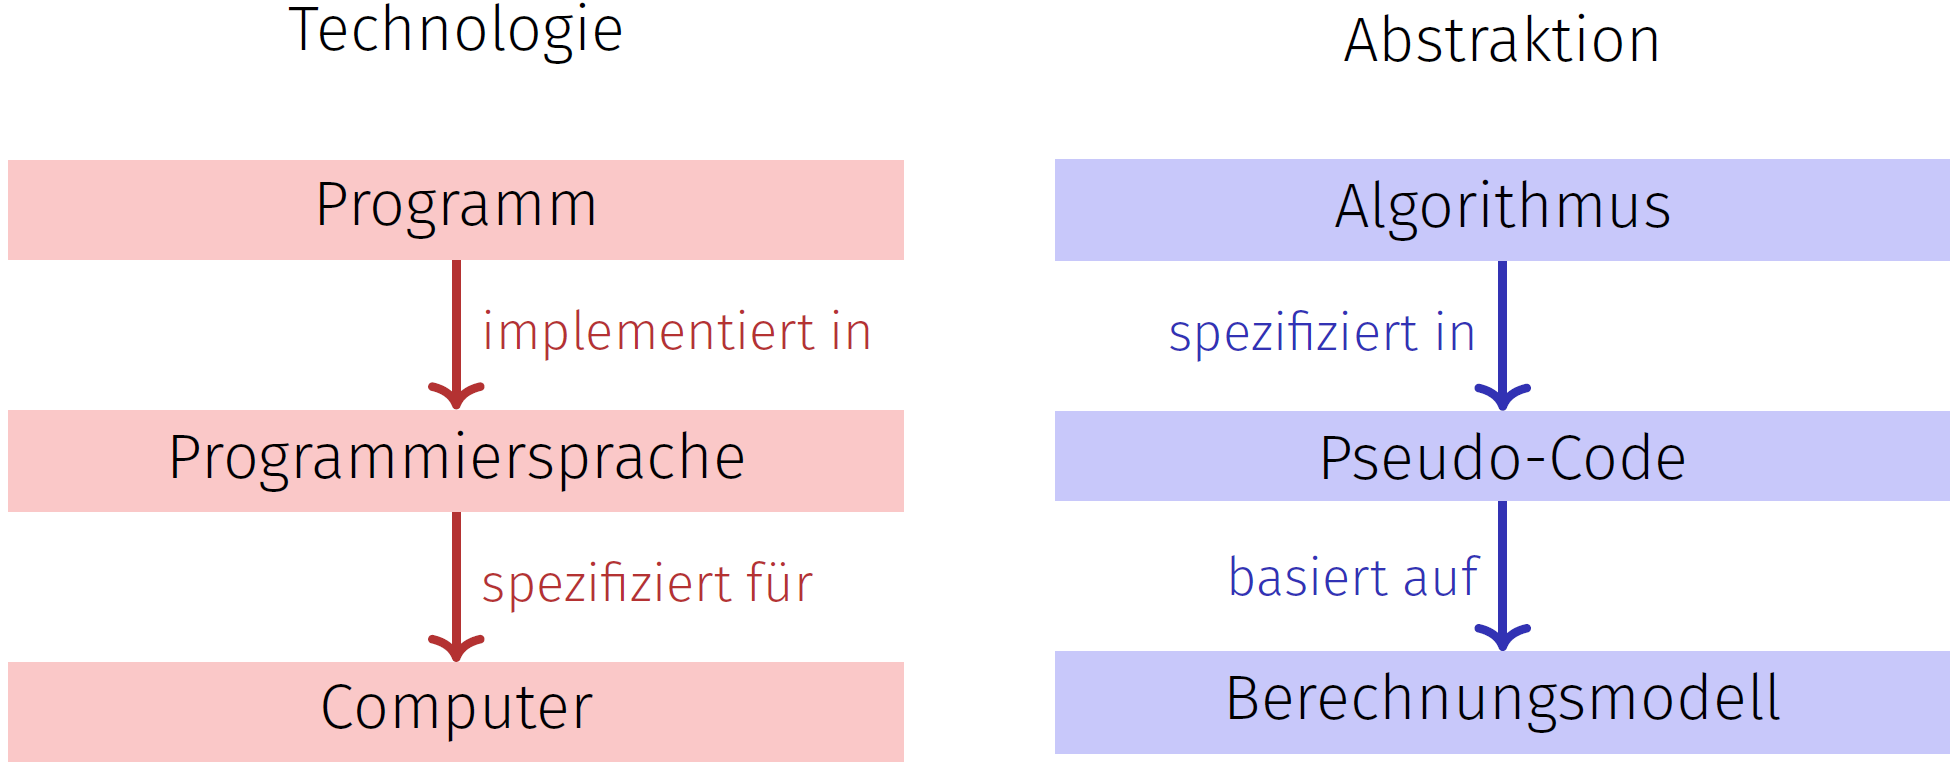
\includegraphics[width = 0.9\columnwidth]{../img/AbstraktionProgramm.png}
%\end{center}\par\smallskip

\textbf{Asymptotische Laufzeiten}\par
\begin{itemize}
    \item \textbf{Obere Schranke}: $\mathcal{O}(g)=\{f:\mathbb{N} \rightarrow \mathbb{R}\ |\ \exists c>0, \exists n_{0} \in \mathbb{N}:$\par $\forall n \geq n_{0}: 0 \leq f(n) \leq c \cdot g(n)\}$
    \item \textbf{Untere Schranke}: $\Omega(g)=\{f: \mathbb{N} \rightarrow \mathbb{R}\ |\ \exists c>0, \exists n_{0} \in \mathbb{N}:$ \par $\forall n \geq n_{0}: 0 \leq c \cdot g(n) \leq f(n)\}$
    \item \textbf{Scharfe Schranke}: $\Theta(g):=\Omega(g) \cap \mathcal{O}(g)$\par
    $\Theta(f) = \{  g: \N \rightarrow \R\ |\ \exists c>0,\ \exists n_0 \in \N:$\par $\forall n \geq n_0: 0 \leq \frac1c \cdot f(n)\leq g(n) \leq c \cdot f(n)\}$
\end{itemize}\par\smallskip

\begin{greenbox}
\textbf{Theorem}\par
Seien $f, g: \mathbb{N} \rightarrow \mathbb{R}^{+}$ zwei Funktionen. Dann gilt.
\begin{enumerate}
    \item $\lim _{n \rightarrow \infty}\limits \frac{f(n)}{g(n)}=0 \Rightarrow f \in \mathcal{O}(g), \mathcal{O}(f) \subsetneq \mathcal{O}(g)$
    \item $\lim _{n \rightarrow \infty}\limits \frac{f(n)}{g(n)}=C>0\ (C \text { konstant}) \Rightarrow f \in \Theta(g)$
    \item $\lim _{n \rightarrow \infty}\limits \frac{f(n)}{g(n)} \longrightarrow \infty \Rightarrow g \in \mathcal{O}(f), \mathcal{O}(g) \subsetneq \mathcal{O}(f)$
\end{enumerate}
\end{greenbox}\smallskip
\textit{Beispiel aufsteigende Laufzeiten:}\par
$ 2^{16},\ \log(n^4),\ \log^8(n),\ \sqrt{n},\ n\log n,\ \binom{n}{3},\ n^5+n,\ \frac{2^n}{n^2},\ n!,\ n^n$\par\smallskip

\textbf{Analyse mit Rekurenz und Teleskopie}\par\vspace{-4px}
\begin{lstlisting}[language=c++]
void g(int n) {
    if (n>1) {
        g(n/2);
        g(n/2);
    }
    else {
        f();
    }
}
\end{lstlisting}\vspace{-4px}
\textit{Rekurrenz} ($n=2^{i}$)\par
$T(n)=\left\{\begin{array}{ll}2 T(n / 2) & n>1 \\ 1 & n=1\end{array}\right.$\par\smallskip
\textit{Teleskopieren}\par
$T(n)=2 \cdot T(n / 2) = 2 \cdot (2 \cdot T(n / 4)) $ \par
$= 2^{i} \cdot T(n/2^{i}) = n \cdot T(n/n) \in \Theta(n)$\par\smallskip

\end{sectionbox}